\documentclass{beamer}
\usepackage[utf8]{inputenc}
\usetheme{Madrid}
\usecolortheme{default}
\usepackage{amsmath,amssymb,amsfonts,amsthm}
\usepackage{txfonts}
\usepackage{tkz-euclide}
\usepackage{listings}
\usepackage{adjustbox}
\usepackage{array}
\usepackage{tabularx}
\usepackage{gvv}
\usepackage{lmodern}
\usepackage{circuitikz}
\usepackage{tikz}
\usepackage{graphicx}

\setbeamertemplate{page number in head/foot}[totalframenumber]

\usepackage{tcolorbox}
\tcbuselibrary{minted,breakable,xparse,skins}



\definecolor{bg}{gray}{0.95}
\DeclareTCBListing{mintedbox}{O{}m!O{}}{%
  breakable=true,
  listing engine=minted,
  listing only,
  minted language=#2,
  minted style=default,
  minted options={%
    linenos,
    gobble=0,
    breaklines=true,
    breakafter=,,
    fontsize=\small,
    numbersep=8pt,
    #1},
  boxsep=0pt,
  left skip=0pt,
  right skip=0pt,
  left=25pt,
  right=0pt,
  top=3pt,
  bottom=3pt,
  arc=5pt,
  leftrule=0pt,
  rightrule=0pt,
  bottomrule=2pt,
  toprule=2pt,
  colback=bg,
  colframe=orange!70,
  enhanced,
  overlay={%
    \begin{tcbclipinterior}
    \fill[orange!20!white] (frame.south west) rectangle ([xshift=20pt]frame.north west);
    \end{tcbclipinterior}},
  #3,
}
\lstset{
    language=C,
    basicstyle=\ttfamily\small,
    keywordstyle=\color{blue},
    stringstyle=\color{orange},
    commentstyle=\color{green!60!black},
    numbers=left,
    numberstyle=\tiny\color{gray},
    breaklines=true,
    showstringspaces=false,
}
%------------------------------------------------------------
%This block of code defines the information to appear in the
%Title page
\title %optional
{2.10.15}

%\subtitle{A short story}

\author % (optional)
{RATHLAVATH JEEVAN -AI25BTECH11026}



\begin{document}


\frame{\titlepage}
\begin{frame}{Question}
The number of vectors of unit length perpendicular to vectors 
\begin{align}
\vec{a} = (1,1,0) \quad \text{and} \quad \vec{b} = (0,1,1)
\end{align}
is
\begin{align}
\text{(a) one \quad (b) two \quad (c) three \quad (d) infinite \quad (e) None of these}
\end{align}
\end{frame}
\begin{frame}{Theoretical Solution} 
Let
\begin{align}
\vec{a}=\myvec{1\\1\\0},\quad 
\vec{b}=\myvec{0\\1\\1}, \quad
\vec{x}=\myvec{x_1\\x_2\\x_3}.
\end{align}
A vector $\vec{x}$ perpendicular to both $\vec{a}$ and $\vec{b}$ satisfies
\begin{align}
\vec{a}^\top\vec{x} &= 0 
\label{eq:q1-ax0}\\
\vec{b}^\top\vec{x} &= 0 
\label{eq:q1-bx0}
\end{align}
\begin{align}
    \begin{myvec}{\vec{a} &&\vec{b}}^T\end{myvec}\vec{x}=\begin{myvec}{0\\0}
    \end{myvec}
\end{align}
From row reduction

\begin{align}
\vec{x}=\lambda\myvec{-1\\1\\-1}.
\label{eq:q1-dir}
\end{align}
\end{frame}
\begin{frame}{Theoretical Solution} 
\textbf{Solution:}\\
Thus a direction vector is
\begin{align}
\vec{n}=\myvec{-1\\1\\-1},\qquad 
\|\vec{n}\|=\sqrt{3}.
\label{eq:q1-norm}
\end{align}
Hence the \emph{unit} vectors perpendicular to both $\vec{a}$ and $\vec{b}$ are
\begin{align}
\vec{u}=\pm\frac{1}{\sqrt{3}}\myvec{-1\\1\\-1}.
\label{eq:q1-unit}
\end{align}
Therefore, the number of such unit vectors is $\boxed{2}$.
\end{frame}
\begin{frame}[fragile]
    \frametitle{C Code}
    \begin{lstlisting}
#include <stdio.h>
#include <math.h>

typedef struct { double x, y, z; } Vec;

Vec cross(Vec a, Vec b) {
    Vec c = {
        a.y*b.z - a.z*b.y,
        a.z*b.x - a.x*b.z,
        a.x*b.y - a.y*b.x
    };
    return c;
}

double norm(Vec v) {
    return sqrt(v.x*v.x + v.y*v.y + v.z*v.z);
}
     \end{lstlisting}
\end{frame}
\begin{frame}[fragile]
    \frametitle{C Code }
    \begin{lstlisting}
Vec scale(Vec v, double s) {
    Vec r = { v.x * s, v.y * s, v.z * s };
    return r;
}

int main(void) {
    // Given vectors
    Vec a = {1, 1, 0};
    Vec b = {0, 1, 1};

    // Vector perpendicular to both is a * b
    Vec n = cross(a, b);
    double m = norm(n);

    // If cross product is zero, vectors are parallel -> infinitely many unit normals
    const double EPS = 1e-12;
    
        
    \end{lstlisting}
    \end{frame}
    \begin{frame}[fragile]
    \frametitle{C Code }
    \begin{lstlisting}
    if (m < EPS) {
        printf("Number of unit vectors perpendicular to both: infinite\n");
        return 0;
        }

    // Two unit vectors:+- (a * b) / ||a * b||
    Vec u = scale(n, 1.0 / m);
    Vec v = scale(u, -1.0);

    printf("Number of unit vectors perpendicular to both: 2\n");
    printf("u1 = (%.6f, %.6f, %.6f)\n", u.x, u.y, u.z);
    printf("u2 = (%.6f, %.6f, %.6f)\n", v.x, v.y, v.z);

    return 0;
}
     \end{lstlisting}
    \end{frame}


\begin{frame}[fragile]
    \frametitle{Python Code}
    \begin{lstlisting}

import numpy as np
import matplotlib.pyplot as plt
from mpl_toolkits.mplot3d import Axes3D

# Given vectors
a = np.array([1, 1, 0])
b = np.array([0, 1, 1])

# Cross product gives a vector perpendicular to both
v = np.cross(a, b)
v = v / np.linalg.norm(v)  # Unit vector

# The two perpendicular unit vectors are +-v
v1 = v
v2 = -v


    \end{lstlisting}
\end{frame}

\begin{frame}[fragile]
    \frametitle{Python Code}
    \begin{lstlisting}
  # Create figure
fig = plt.figure()
ax = fig.add_subplot(111, projection='3d')

# Plot given vectors
ax.quiver(0, 0, 0, a[0], a[1], a[2], color='r', label='a = (1,1,0)')
ax.quiver(0, 0, 0, b[0], b[1], b[2], color='g', label='b = (0,1,1)')

# Plot perpendicular unit vectors
ax.quiver(0, 0, 0, v1[0], v1[1], v1[2], color='b', label='Unit perp vector +v')
ax.quiver(0, 0, 0, v2[0], v2[1], v2[2], color='orange', label='Unit perp vector -v')

    \end{lstlisting}
\end{frame}

\begin{frame}[fragile]
    \frametitle{Python Code}
    \begin{lstlisting}
# Set labels
ax.set_xlabel('X')
ax.set_ylabel('Y')
ax.set_zlabel('Z')
ax.set_title('Unit vectors perpendicular to a and b')
ax.legend()

# Save image
plt.savefig("perpendicular_vectors.png")
plt.show()
    \end{lstlisting}
\end{frame}

\begin{frame}{Plot}
    \centering
    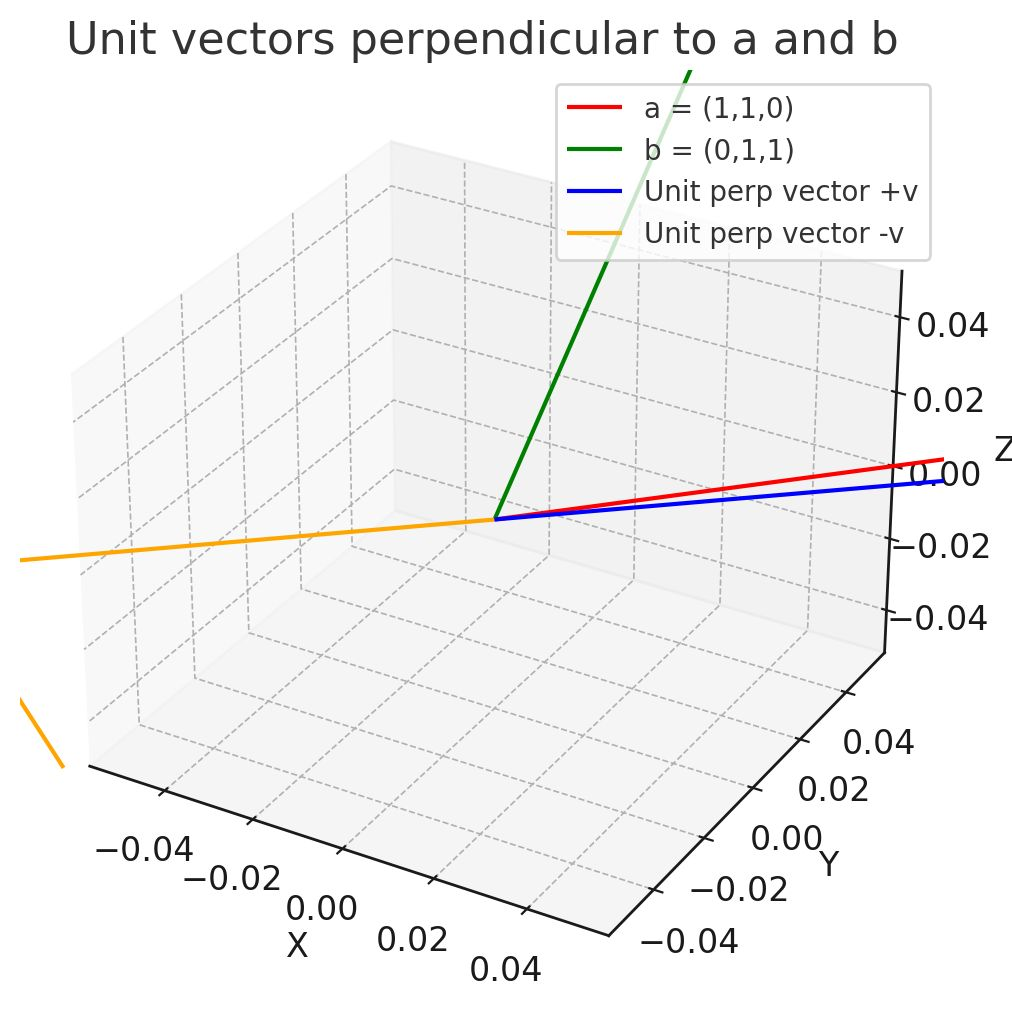
\includegraphics[width=\columnwidth, height=0.8\textheight, keepaspectratio]{beamer/figs/matg5.jpeg}     
\end{frame}




\end{document}
